\chapter{Teil 2: Klassifikation}
\section{Einleitung}
Um eine Klassifizierung durchführen zu können, sind mehrere Komponenten notwendig, welche miteinander arbeiten. 
Dieser Ablauf wird in der \cref{fig:ablauf_klassifizierung} gezeigt.
\begin{figure}[H]	
	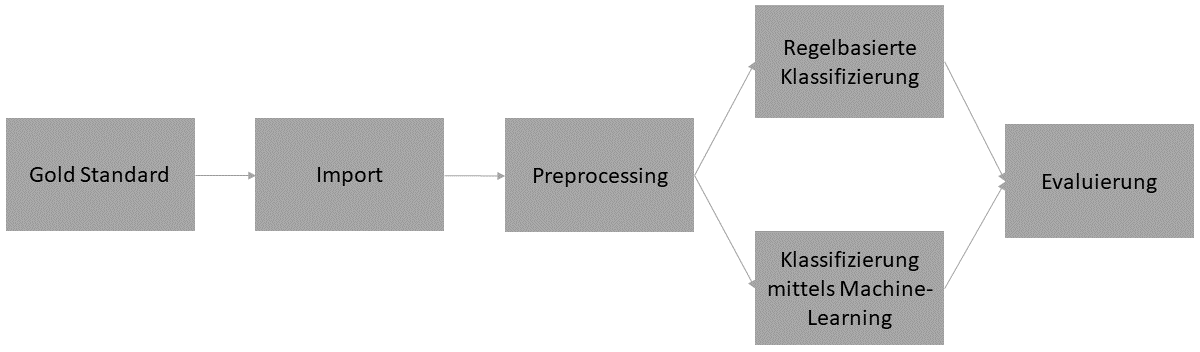
\includegraphics[width=1\columnwidth,keepaspectratio]{img/Ablauf_Klassifizierung.png}
	\caption{Pipeline}
	\label{fig:ablauf_klassifizierung}
\end{figure}
Als Grundlage dienen die Daten des Gold Standards.
Diese werden mittels einer Import-Komponente geladen.
Bevor die Daten mit den entsprechenden Methoden klassifiziert werden, werden sie bei Bedarf noch vorverarbeitet.
Dann findet die eigentliche Klassifizierung statt.
Um eine möglichst präzise und erfolgreiche Variante des Klassifizierens zu finden, werden in diesem Teil der Arbeit mehrere Experimente durchgeführt.
Zum Schluss folgt eine Komponente, welche für das Auswerten der Klassifizierung und Ausgeben der Ergebnisse verantwortlich ist.
\section{Preprocessing}
Das Preprocessing wurde entwickelt, um den Inhalt des Dokuments auf eine standardisierte Form zu bringen.
Die folgenden Methoden können sowohl auf den Text eines Dokuments sowie auch auf den Titel angewendet werden.
Sie können mittels Konfiguration sowohl für den Text als auch Titel eines Dokuments ein- oder ausgeschaltet werden.
\subsection{Basis Preprocessing}
\subsubsection{Gross-/Kleinschreibung}
Alle Buchstaben, welche grossgeschrieben sind, werden durch die entsprechenden Kleinbuchstaben ersetzt.
\subsubsection{Umlaute ersetzen}
Umlaute werden durch ihre verwandten Selbstlaute ersetzt, genauer:
\begin{itemize}
	\item ä $\rightarrow$ a
	\item ö $\rightarrow$ o
	\item ü $\rightarrow$ u
\end{itemize} 
\subsubsection{Sonderzeichen entfernen}
Alle Sonderzeichen, die nicht in der folgenden Auflistung vorkommen, werden durch einen Leerschlag ersetzt:
\begin{itemize}
	\item éàèÉÀÈäöüÄÖÜa-zA-Z
\end{itemize} 
\subsubsection{Einzelne Zeichen entfernen}
Jedes einzelne Zeichen, also solche, die sowohl vorne als auch hinten an einen Leerschlag angrenzen, werden entfernt.
\subsubsection{Multiple Leerschläge entfernen}
Da durch die vorhergehenden Schritte oft multiple Leerschläge anfallen, werden diese auf einen Leerschlag reduziert.
\subsection{Erweiterte Preprocessing}
\subsubsection{Preisdetektor}
Da Menüs häufig in Verbindung mit Preisen vorkommen und in weiteren Preprocessing-Schritten Zahlen und Sonderzeichen entfernt werden, ist es von Vorteil, diese Informationen nicht zu verlieren.
Daher erkennt diese Methode verschiedene Varianten von Preisen mittels Regulären Ausdrücken (Regex, Regular Expression) und ersetzt diese mit einem Schlüsselwort.
% Varianten genauer ausführen
Die folgenden Varianten von Preisen wird erkannt:
\begin{itemize}
	\item Preisangabe + chf/fr/sfr
	\item Preisangabe
	\item chf/fr/sfr + Preisangabe
\end{itemize} 
Zudem wird unterschieden, wie viele Stellen der Preis hat.
Die nun aufgeführte Liste zeigt die verschiedenen Schlüsselwörter:
\begin{itemize}
	\item Einstellig $\rightarrow$ onedigitprice
	\item Zweistellig $\rightarrow$ twodigitprice
	\item Dreistellig $\rightarrow$ threedigitprice
\end{itemize} 
Um Zeitangaben nicht als Preise zu erkennen, werden bei Preisangaben ohne Währungsangabe nur Beträge mit Rappenbeträgen, welche 60 oder höher sind, erkannt.
\subsubsection{Stammformreduktion}
Dieses Verfahren führt verschiedene morphologische Varianten eines Wortes auf ihren gemeinsamen Stamm zurück.
Dafür wird der Stemmer \glqq Cistem\footnote{\url{https://github.com/LeonieWeissweiler/CISTEM} abgerufen am: 18.03.2019}\grqq{} verwendet, da für die deutsche Sprache nur wenig Alternativen vorhanden sind. 
\subsubsection{Getränkedetektor}
% Referenz Cistem
Eine Liste mit Einträgen diverser Getränke bildet die Grundlage dieser Methode.
Wenn im Text ein Getränk dieser Liste vorhanden ist, wird es durch das Schlüsselwort \glqq beverageentity\grqq{} ersetzt.
Damit soll erreicht werden, dass ein einheitliches Merkmal geschaffen wird.
\subsubsection{Stoppwörter entfernen}
Bei Stoppwörter handelt es sich um Wörter, welche keine Relevanz für den Inhalt eines Texts haben, aber oft vorkommen.
Eine Stoppwortliste führt 1720 solcher Wörter in deutsch auf. Sie ist aus mehreren Quellen zusammengesetzt worden.
Wenn eines dieser Wörter im Text vorkommt, wird es entfernt.
Die Experimente sind auf dem Trainings-Datensatzes des Gold Standards durchgeführt worden.
Die schlussendlichen Resultate wurden anhand des Test-Datensatzes dessen durchgeführt.
\section{Regelbasierte Experimente}
\subsection{Regelsatz: Menü im Titel}
\subsubsection{Beschreibung der Komponente}
Dieser simple Algorithmus kontrolliert, ob das Wort \glqq menu\grqq{} im Metatag \glqq Title\grqq{} vorkommt.
Falls ja, wird das Dokument als Menüseite klassiert.
\subsubsection{Methoden}
Für dieses Regelset sind keine Parameter verfügbar, daher ist nur eine Konfiguration durchgeführt worden.
Diese hat folgende Metriken ergeben:\\
\begin{table}[H]
	\caption{Score des Regelsets: Menü im Titel}
	\centering
	\begin{tabular}{|l|l|l|}
		\hline
		F1-Score & Precision & Recall\\
		\hline
		0.17 & 0.43 & 0.11  \\
		\hline
	\end{tabular}
\end{table}
\subsubsection{Resultate}
Das folgende Ergebnis ist anhand der Daten des Testsets entstanden:
\begin{table}[H]
	\caption{Beste Scores des Regelsatzes: Menü im Titel}
	\centering
	\begin{tabular}{|l|l|l|l|}
		\hline
		Methode & F1-Score & Precision & Recall\\
		\hline
		Menü im Titel & 0.28 & 1.00 & 0.16 \\
		\hline
	\end{tabular}
\end{table}
Die Klassifizierung in absoluten Zahlen wird mittels Konfusionsmatrix verdeutlicht.
\begin{table}[H]
	\caption{Konfusionsmatrix des Regelsets: Menü im Titel}
	\centering
	\begin{tabular}{@{}cc|cc@{}}
		\multicolumn{1}{c}{} &\multicolumn{1}{c}{} &\multicolumn{2}{c}{Predicted} \\ 
		\multicolumn{1}{c}{} & 
		\multicolumn{1}{c|}{} & 
		\multicolumn{1}{c}{Positiv} & 
		\multicolumn{1}{c}{Negativ} \\ 
		\cline{2-4}
		\multirow[c]{2}{*}{\rotatebox[origin=tr]{90}{Actual}}
		& Positiv  & 8   & 42   \\[1.5ex]
		& Negativ  & 0   & 50 \\ 
		\cline{2-4}
	\end{tabular}
\end{table}
\subsection{Regelsatz: Preisdetektor}
\subsubsection{Beschreibung der Komponente}
Dieser Algorithmus funktioniert dank der Preprocessing-Methode, welche den Preis erkennt und mit einem Schlüsselwort ersetzt.
Sofern dieses Schlüsselwort im Text vorhanden ist, wird das Dokument als Menüseite klassifiziert. Dies unter der Annahme, dass Menüpreise oft zweistellig sind, im Gegensatz zu Getränkepreisen welche häufig einstellig sind und Hotelpreisen, die meist dreistellig sind.
Die Anzahl vorhandener Preise kann über die Konfiguration angegeben werden.
\subsubsection{Methoden}
Durch die Konfiguration kann ein Schwellwert für die Anzahl erkannter Preise angegeben werden, die vorhanden sein müssen, um eine Webpage als positiv zu klassifizieren.\\
\begin{table}[H]
	\caption{Scores des Regelsets: Preisdetektor}
	\centering
	\begin{tabular}{|l|l|l|l|}
		\hline
		Schwellwert & F1-Score & Precision & Recall\\
		\hline
		1 & 0.45 & 0.36 & 0.60  \\
		2 & 0.46 & 0.45 & 0.47 \\
		3 & 0.41 & 0.49 & 0.36 \\
		\hline
	\end{tabular}
\end{table}
Das beste Ergebnis hat ein Schwellwert von zwei erzielt, danach ist der F1-Score wieder schlechter geworden.
Daraus wurde geschlussfolgert, dass für dieses Regelset das Maximum bereits erreicht wurde.
\subsubsection{Resultate}
Das folgende Ergebnis ist anhand der Daten des Testsets entstanden:
\begin{table}[H]
	\caption{Beste Scores des Regelsatzes: Menü im Titel}
	\centering
	\begin{tabular}{|l|l|l|l|}
		\hline
		Methode & F1-Score & Precision & Recall\\
		\hline
		Preisdetektor & 0.65 & 0.93 & 0.50 \\
		\hline
	\end{tabular}
\end{table}
Die Klassifizierung in absoluten Zahlen wird mittels Konfusionsmatrix verdeutlicht.
\begin{table}[H]
	\caption{Konfusionsmatrix des Regelsets: Preisdetektor}
	\centering
	\begin{tabular}{@{}cc|cc@{}}
		\multicolumn{1}{c}{} &\multicolumn{1}{c}{} &\multicolumn{2}{c}{Predicted} \\ 
		\multicolumn{1}{c}{} & 
		\multicolumn{1}{c|}{} & 
		\multicolumn{1}{c}{Positiv} & 
		\multicolumn{1}{c}{Negativ} \\ 
		\cline{2-4}
		\multirow[c]{2}{*}{\rotatebox[origin=tr]{90}{Actual}}
		& Positiv  & 25   & 25   \\[1.5ex]
		& Negativ  & 2    & 48 \\ 
		\cline{2-4}
	\end{tabular}
\end{table}
\subsection{Regelsatz: Kombination aus Menü im Titel und Preisdetektor}
\subsubsection{Beschreibung der Komponente}
Diese Kombination führt eine sequenzielle Klassifikation aus.
Im ersten Schritt wird der Mechanismus des Algorithmus \glqq Menü im Titel\grqq{} verwendet.
Falls durch diesen keine positive Klassifikation zustande kommt, wird durch den Preisdetektor nochmals neu klassifiziert.
\subsubsection{Methoden}
Bei dieser Konfiguration kann der Schwellwert ebenfalls für die Anzahl erkannter Preise angegeben werden.\\
\begin{table}[H]
	\caption{Scores des Regelsets: Kombination aus Menü im Titel und Preisdetektor}
	\centering
	\begin{tabular}{|l|l|l|l|}
		\hline
		Schwellwert & F1-Score & Precision & Recall\\
		\hline
		1 & 0.45 & 0.35 & 0.65 \\
		2 & 0.47 & 0.43 & 0.52 \\
		3 & 0.43 & 0.45 & 0.41 \\
		\hline
	\end{tabular}
\end{table}
Auch bei diesem Regelset hat die Konfiguration mit einem Schwellwert von zwei das beste Ergebnis erzielt.
\subsubsection{Resultate}
Das folgende Ergebnis ist anhand der Daten des Testsets entstanden:
\begin{table}[H]
	\caption{Beste Scores des Regelsatzes: Menü im Titel}
	\centering
	\begin{tabular}{|l|l|l|l|}
		\hline
		Methode & F1-Score & Precision & Recall\\
		\hline
		Kombination aus Menü im Titel und Preisdetektor & 0.70 & 0.93 & 0.56\\
		\hline
	\end{tabular}
\end{table}
Die Klassifizierung in absoluten Zahlen wird mittels Konfusionsmatrix verdeutlicht.
\begin{table}[H]
	\caption{Konfusionsmatrix des Regelsets: Kombination aus Menü im Titel und Preisdetektor}
	\centering
	\begin{tabular}{@{}cc|cc@{}}
		\multicolumn{1}{c}{} &\multicolumn{1}{c}{} &\multicolumn{2}{c}{Predicted} \\ 
		\multicolumn{1}{c}{} & 
		\multicolumn{1}{c|}{} & 
		\multicolumn{1}{c}{Positiv} & 
		\multicolumn{1}{c}{Negativ} \\ 
		\cline{2-4}
		\multirow[c]{2}{*}{\rotatebox[origin=tr]{90}{Actual}}
		& Positiv  & 28   & 22   \\[1.5ex]
		& Negativ  & 2   & 48 \\ 
		\cline{2-4}
	\end{tabular}
\end{table}
\subsection{Regelsatz: Listing}
\subsubsection{Beschreibung der Komponente}
Dieser Algorithmus basiert sowohl auf dem Black- als auch auf dem Whitelisting Ansatz.
Dazu wird eine Blacklist und eine Whitelist verwendet, die von Hand erstellt wurden und Einträge enthalten, welche für die jeweiligen Kategorien typisch sind.
Falls ein Wort einer Liste im Text einer Webpage vorkommt, wird ein entsprechender Zähler hochgezählt.
Zum Schluss findet eine sequenzielle Klassifizierung statt, das heisst: 
Wenn der Zähler der Blacklist einen konfigurierbaren Schwellwert überschreitet, wird die Webpage als negativ klassifiziert. 
Wenn der Zähler der Whitelist einen konfigurierbaren Schwellwert überschreitet, wird die Webpage als Menüseite klassifiziert.
Falls keiner der beiden Zähler den Schwellwert überschreitet, wird die Webpage ebenfalls als negativ klassifiziert. 
\subsubsection{Methoden}
Beim Listing können zwei Schwellwerte angeben werden, einen für die Anzahl übereinstimmender Wörter aus der Whitelist und einen für die Blacklist.
In einem ersten Versuch wurden identische Schwellwerte gewählt und jeweils erhöht:\\
\begin{table}[H]
	\caption{Scores der ersten Iteration des Regelsets: Listing}
	\centering
	\begin{tabular}{|l|l|l|l|l|}
		\hline
		Schwellwert Whitelist & Schwellwert Blacklist & F1-Score & Precision & Recall\\
		\hline
		1 & 1 & 0.17 & 0.32 & 0.11 \\
		5 & 5 & 0.39 & 0.62 & 0.29 \\
		10 & 10 & 0.42 & 0.77 & 0.29 \\
		20 & 20 & 0.33 & 0.85 & 0.21 \\
		30 & 30 & 0.27 & 0.91 & 0.16 \\
		\hline
	\end{tabular}
\end{table}
Dieser Versuch hat gezeigt, dass ein maximaler F1-Score bei gleichen Werten zwischen 5 und 20 zu erreichen ist.\\
Da gleich gewählte Werte keine zufriedenstellende Ergebnisse erzielten, wurden im zweiten Versuch unterschiedliche Verhältnisse getestet:\\
\begin{table}[H]
	\caption{Scores der zweiten Iteration des Regelsets: Listing}
	\centering
	\begin{tabular}{|l|l|l|l|l|}
		\hline
		Schwellwert Whitelist & Schwellwert Blacklist & F1-Score & Precision & Recall\\
		\hline
		5 & 1 & 0.12 & 0.82 & 0.07 \\
		1 & 5 & 0.31 & 0.24 & 0.45 \\
		\hline
	\end{tabular}
\end{table}
Aus diesem Versuch entstand die Schlussfolgerung, dass ein höherer Schwellwert der Blacklist als der Whitelist erforderlich ist, um einen möglichst hohen Score zu erreichen.
Diese Erkenntnis wurde in einem weiteren Versuch in mehreren Iterationen getestet:\\
\begin{table}[H]
	\caption{Scores der dritten Iteration des Regelsets: Listing}
	\centering
	\begin{tabular}{|l|l|l|l|l|}
		\hline
		Schwellwert Whitelist & Schwellwert Blacklist & F1-Score & Precision & Recall\\
		\hline
		2 & 10 & 0.42 & 0.33 & 0.61 \\
		3 & 15 & 0.52 & 0.42 & 0.70 \\
		3 & 20 & 0.51 & 0.39 & 0.75 \\
		4 & 15 & 0.53 & 0.47 & 0.61 \\
		5 & 15 & 0.55 & 0.54 & 0.56 \\
		5 & 20 & 0.54 & 0.50 & 0.60 \\
		5 & 21 & 0.54 & 0.49 & 0.60 \\
		6 & 20 & 0.55 & 0.56 & 0.55 \\
		7 & 20 & 0.55 & 0.60 & 0.50 \\
		8 & 20 & 0.53 & 0.64 & 0.46 \\
		\hline
	\end{tabular}
\end{table}
Die Schwellwerte wurden stetig erhöht.
Verschiedene Schwellwerte in unterschiedlichen Verhältnissen wurden dabei getestet.
Sobald einer dieser Schwellwerte zu einem schlechteren Ergebnis geführt hat, wurde er wieder reduziert oder ein neues Verhältnis wurde getestet.
Beim Verhältnis 6/20 bzw. 7/20 wurde das Maximum des F1-Scores erreicht.
Da diese Werte nicht im Bereich einer zufriedenstellenden Klassifikation sind, wurde auf das Ermitteln aller möglichen Kombinationen verzichtet.
\subsubsection{Resultate}
Das folgende Ergebnis ist anhand der Daten des Testsets entstanden:
\begin{table}[H]
	\caption{Beste Scores des Regelsatzes: Menü im Titel}
	\centering
	\begin{tabular}{|l|l|l|l|}
		\hline
		Methode & F1-Score & Precision & Recall\\
		\hline
		Listing & 0.68 & 0.96 & 0.52\\
		\hline
	\end{tabular}
\end{table}
Die Klassifizierung in absoluten Zahlen wird mittels Konfusionsmatrix verdeutlicht.
\begin{table}[H]
	\caption{Konfusionsmatrix des Regelsets: Listing}
	\centering
	\begin{tabular}{@{}cc|cc@{}}
		\multicolumn{1}{c}{} &\multicolumn{1}{c}{} &\multicolumn{2}{c}{Predicted} \\ 
		\multicolumn{1}{c}{} & 
		\multicolumn{1}{c|}{} & 
		\multicolumn{1}{c}{Positiv} & 
		\multicolumn{1}{c}{Negativ} \\ 
		\cline{2-4}
		\multirow[c]{2}{*}{\rotatebox[origin=tr]{90}{Actual}}
		& Positiv  & 26   & 24   \\[1.5ex]
		& Negativ  & 1   & 49 \\ 
		\cline{2-4}
	\end{tabular}
\end{table}
\subsection{Regelsatz: Bag of Words}
\subsubsection{Beschreibung der Komponente}
Dieser Algorithmus basiert auf dem statistischen Ansatz namens \glqq Bag of Words\grqq{}.
Dafür wird der komplette Datensatz in einen Trainings- und Testsatz in einem konfigurierbaren Verhältnis aufgeteilt.
Bag of Words zählt für jedes Dokument der Trainingsdaten, wie oft ein Wort darin vorkommt.
In dieser Anwendung wird jedoch nur erkannt, ob ein Wort vorkommt, oder nicht, die Anzahl spielt keine Rolle.
Anhand dieser Wörter wird eine dynamische Black- und Whitelist erstellt, Wörter die in beiden Listen vorkommen, werden entfernt.
Anhand dieser Listen wird der Testdatensatz klassifiziert.
Die Anzahl der Wörter dieser Listen ist konfigurierbar.
Die Klassifikation findet mittels einem Zähler statt.
Für jedes Wort eines Dokuments, welches in der Liste der positiven Beispielen vorkommt, wird der Zähler hochgezählt, für jedes Wort aus der Liste der negativen Beispielen wird er heruntergezählt.
Für die Klassifizierung wird der Zähler mit einem konfigurierbaren Schwellwert verglichen, Falls der Zähler grösser ist als der Schwellwert, wird das Dokument als positiv klassifiziert, ansonsten negativ.
Um die Ergebnisse anhand der Testdaten evaluieren zu können, sind diese Listen zudem statisch implementiert worden.
Ob diese dynamisch erzeugt werden oder die statisch implementierten Listen verwendet werden sollen, kann mittels Konfigurationsoption gewählt werden.
\subsubsection{Methoden}
Bei diesem Regelset kann die Grösse der Black- und Whitelist (Features), das Verhältnis zwischen Test- und Trainingsdaten (Split) sowie ein Schwellwert angegeben werden.
Für das Verhältnis zwischen Test- und Trainingsdaten wurden die Werte 0.3, 0.5 und 0.7 getestet.
In einer ersten Iteration wurde die Anzahl von 200 Features und ein Split von 0.3 verwendet, um herauszufinden, ob ein positiver oder negativer Schwellwert bessere Werte erzielt.\\
\begin{table}[H]
	\caption{Scores der ersten Iteration des Regelsets: Bag of Words}
	\centering
	\begin{tabular}{|l|l|l|l|}
		\hline
		Schwellwert & F1-Score & Precision & Recall\\
		\hline
		0 & 0.64 & 0.58 & 0.71 \\
		2 & 0.51 & 0.38 & 0.75 \\
		-2 & 0.68 & 0.74 & 0.63 \\
		\hline
	\end{tabular}
\end{table}
Dabei wurde erkannt, dass sich ein negativer Schwellwert positiv auf den F1-Score auswirkt.\\
In der zweiten Iteration wurde der Schwellwert weiter verkleinert.\\
\begin{table}[H]
	\caption{Scores der zweiten Iteration des Regelsets: Bag of Words}
	\centering
	\begin{tabular}{|l|l|l|l|}
		\hline
		Schwellwert & F1-Score & Precision & Recall\\
		\hline
		-3 & 0.66 & 0.80 & 0.57 \\
		-4 & 0.66 & 0.86 & 0.54 \\
		-5 & 0.66 & 0.89 & 0.52 \\
		\hline
	\end{tabular}
\end{table}\
Da diese Werte sich fast nicht unterscheiden, wurden alle weiterverwendet, um einen maximalen Score zu evaluieren.
In einer dritten, ausführlicheren Iteration sind die Anzahl Features von 200 bis 400 sowie die drei oben genannten Verhältnisse zusammen mit den vier Schwellwerten getestet worden. Die Tabelle \cref{tab:bow3} zeigt diese Tests, sortiert nach bestem F1-Score:\\
\FloatBarrier
\begin{table}
	\caption{Scores der dritten Iteration des Regelsets: Bag of Words}
	\centering
	\label{tab:bow3}
	\begin{tabular}{ | l | l | l | l | l | l | }
		\hline
		Split & Features & Limit & F1-Score & Precision & Recall \\ \hline
		0.3 & 400 & -3 & 0.72 & 0.74 & 0.7 \\ 
		0.3 & 400 & -4 & 0.72 & 0.79 & 0.66 \\
		0.3 & 400 & -5 & 0.72 & 0.81 & 0.64 \\
		0.7 & 400 & -3 & 0.72 & 0.75 & 0.69 \\
		0.7 & 400 & -4 & 0.72 & 0.79 & 0.66 \\
		0.5 & 300 & -3 & 0.71 & 0.79 & 0.65 \\
		0.5 & 400 & -3 & 0.70 & 0.74 & 0.67 \\
		0.5 & 400 & -4 & 0.70 & 0.79 & 0.63 \\ 
		0.7 & 400 & -2 & 0.70 & 0.70 & 0.70 \\ 
		0.7 & 300 & -3 & 0.70 & 0.74 & 0.67 \\
		0.7 & 300 & -4 & 0.70 & 0.80 & 0.63 \\
		0.7 & 300 & -5 & 0.70 & 0.84 & 0.60 \\
		0.7 & 400 & -5 & 0.70 & 0.82 & 0.62 \\ 
		0.3 & 400 & -2 & 0.69 & 0.66 & 0.73 \\ 
		0.5 & 400 & -2 & 0.69 & 0.69 & 0.69 \\ 
		0.5 & 400 & -5 & 0.69 & 0.82 & 0.60 \\ 
		0.7 & 200 & -3 & 0.69 & 0.76 & 0.63 \\ 
		0.7 & 200 & -4 & 0.69 & 0.81 & 0.60 \\ 
		0.3 & 300 & -2 & 0.68 & 0.73 & 0.64 \\ 
		0.3 & 300 & -3 & 0.68 & 0.78 & 0.60 \\ 
		0.3 & 200 & -2 & 0.68 & 0.74 & 0.63 \\ 
		0.5 & 200 & -3 & 0.68 & 0.77 & 0.60 \\ 
		0.5 & 300 & -4 & 0.68 & 0.81 & 0.59 \\ 
		0.7 & 300 & -2 & 0.68 & 0.69 & 0.68 \\ 
		0.5 & 200 & -2 & 0.67 & 0.71 & 0.64 \\ 
		0.3 & 300 & -4 & 0.66 & 0.82 & 0.56 \\ 
		0.3 & 200 & -3 & 0.66 & 0.80 & 0.57 \\
		0.3 & 200 & -4 & 0.66 & 0.86 & 0.54 \\
		0.3 & 200 & -5 & 0.66 & 0.89 & 0.52 \\ 
		0.5 & 200 & -4 & 0.66 & 0.81 & 0.56 \\
		0.5 & 300 & -5 & 0.66 & 0.83 & 0.55 \\ 
		0.7 & 200 & -2 & 0.66 & 0.66 & 0.66 \\ 
		0.7 & 200 & -5 & 0.66 & 0.85 & 0.55 \\ 
		0.3 & 300 & -5 & 0.65 & 0.85 & 0.52 \\ 
		0.5 & 200 & -5 & 0.65 & 0.87 & 0.52 \\
		0.5 & 300 & -2 & 0.46 & 0.62 & 0.36 \\ \hline
	\end{tabular}
\end{table}
Daraus lässt sich schliessen, dass eine hohe Anzahl Features zu einem besseren Ergebnis führt.
Das Verhältnis zwischen Test- und Trainingsdaten ist nicht so relevant, da sowohl das Verhältnis 0.3 als auch 0.7 zu hohen Scores führt.
Der Schwellwert ist im Bereich -2 bis -5 ebenfalls nicht aussagekräftig, da auch dieser bei den besten Scores vertreten ist.
Es muss zudem berücksichtigt werden, dass der Split zufällig gewählt wird und keine Kreuzvalidierung stattfindet, dadurch können diese Ergebnisse variieren.
\FloatBarrier
\subsubsection{Resultate}
Das folgende Ergebnis ist anhand der Daten des Testsets entstanden:\\
\begin{table}[H]
	\caption{Beste Scores des Regelsatzes: Menü im Titel}
	\centering
	\begin{tabular}{|l|l|l|l|}
		\hline
		Methode & F1-Score & Precision & Recall\\
		\hline
		Bag of Words & 0.74 & 0.91 & 0.62\\
		\hline
	\end{tabular}
\end{table}
Die Klassifizierung in absoluten Zahlen wird mittels Konfusionsmatrix verdeutlicht.
\begin{table}[H]
	\caption{Konfusionsmatrix des Regelsets: Bag of Words}
	\centering
	\begin{tabular}{@{}cc|cc@{}}
		\multicolumn{1}{c}{} &\multicolumn{1}{c}{} &\multicolumn{2}{c}{Predicted} \\ 
		\multicolumn{1}{c}{} & 
		\multicolumn{1}{c|}{} & 
		\multicolumn{1}{c}{Positiv} & 
		\multicolumn{1}{c}{Negativ} \\ 
		\cline{2-4}
		\multirow[c]{2}{*}{\rotatebox[origin=tr]{90}{Actual}}
		& Positiv  & 31   & 19   \\[1.5ex]
		& Negativ  & 3   & 47 \\ 
		\cline{2-4}
	\end{tabular}
\end{table}
\subsection{Diskussion der regelbasierten Experimente}
\section{Experimente mittels Machine-Learning}
\subsection{Dimensionsreduktion der Features}
\subsubsection{Beschreibung der Komponente}
\subsubsection{Methoden}
\subsubsection{Resultate}
\subsection{Angabe von Klassenverteilung}
\subsubsection{Beschreibung der Komponente}
\subsubsection{Methoden}
\subsubsection{Resultate}
\subsection{Anwendung von N-Gramme}
\subsubsection{Beschreibung der Komponente}
\subsubsection{Methoden}
\subsubsection{Resultate}
\subsection{Anwendung von einfachen Preprocssingschritten}
\subsubsection{Beschreibung der Komponente}
\subsubsection{Methoden}
\subsubsection{Resultate}
\subsection{Anwendung von fortgeschrittenen Preprocssingschritten}
\subsubsection{Beschreibung der Komponente}
\subsubsection{Methoden}
\subsubsection{Resultate}
\subsection{Anzahl extrahierter Features}
\subsubsection{Beschreibung der Komponente}
\subsubsection{Methoden}
\subsubsection{Resultate}
\subsection{Hyperparametertuning}
\subsubsection{Beschreibung der Komponente}
\subsubsection{Methoden}
\subsubsection{Resultate}
\subsection{Diskussion der regelbasierten Experimente}
\section{Diskussion}
\section{Beantwortung der Forschungsfrage}
\section{Verwendete Technologien}